\section{Early Work}
Early steps I was advised to work on was, getting an idea of \emph{learning} in two dimensions (2D) to get an intuition and follow it on with expanding it to three dimensions (3D) from there.

\subsection{Structuring the Problem}
Following those ideas I wanted to create a simple task to train a policy to teach a block to move towards the other block, on simple 2D rendered canvas. Essentially creating a two dimensional reaching task.

\subsubsection{Designing the Problem} 
I started with pygame \cite{pygame}, a python library that can be used to create 2D canvas with artifacts in it. But before rendering there are some things we have to define. I wanted to create a small\emph{ish} canvas to simulate the game in, with my player and target. I chose to make a $800 \times 600$ canvas and defined my blocks to be $20 \times 20$. Skipping the details the simple game was rendered as Figure \ref{fig:initial-canvas}, where the agent (blue) attempts to get to the target (red).

\begin{figure}[h]
  \centering
  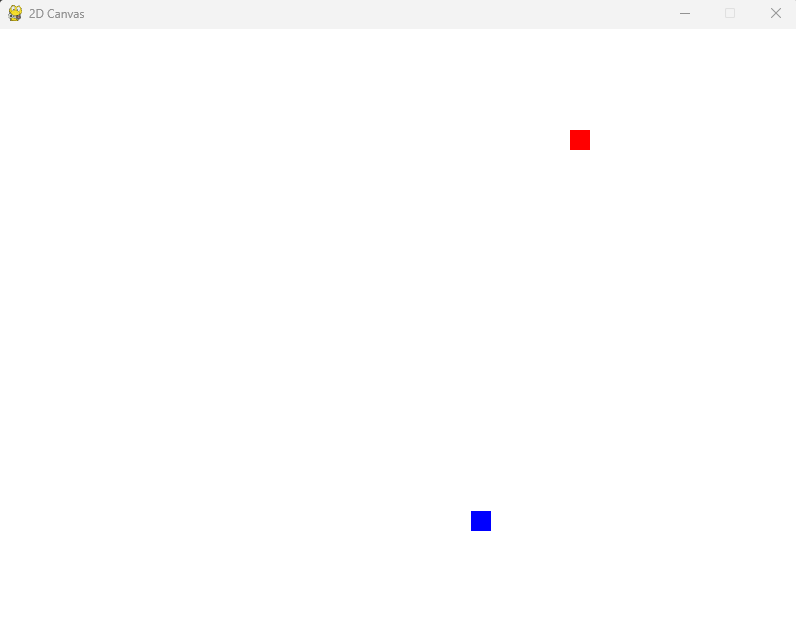
\includegraphics[width=0.6\textwidth]{assets/early-work/initial-canvas.png}
  \caption{Initial canvas $800 \times 600$ and $20 \times 20$ blocks}\label{fig:initial-canvas}
\end{figure}

As this was a simple game, for movement I defined a speed, which was initially $5$ pixels per press and mapped the movements to the arrow keys, and wrote a simple check that when the agent makes it to the target the game is complete.

\subsection{Solving the Problem: Learning}
To make a policy that would play the game, there was a few things I needed; firstly, the game needed a model to solve, I started with a classificiation approach, to classify the correct keys to press to move to the target.


\subsubsection{Classification}
Therefore, my model was fairly simple; the state, $S$ which is a \emph{4-tuple} $\langle float, float, float, float \rangle$ that holds -in order- $x$-coordinate of agent, $y$-coordinate of agent, $x$-coordinate of target and the $y$-coordinate of target. And due to the keypress nature of the system, the Action, $\mathcal{A}$ was also a \emph{4-tuple} $\langle boolean, boolean, boolean, boolean \rangle$ which was true or false to indicate if an arrow key was pressed, the positions in order are: \emph{Up, Down, Left} and \emph{Right}.

So, Using this knowing the space, I created an expert policy, \(\pi_{demo}\), which gives the key combinations that must be pressed by interpolating where the target is with respect to the agent. Using their coordinates this was pretty simple. So, I randomly generated some starting positions and made the agent play the game many times and got snapshots of the states and stored them in a labelled structure for training a model later. \(data: list\left[State, Action\right]\) where:
\[
  State: tuple\left[float, float, float, flaot\right], 
  \hspace{1cm} Action: tuple\left[bool, bool, bool, bool\right]
\]
as before. (Data loading was managed with dataframes and pickles for optimal GPU loading and speed)

Therefore, combining the two, I trained a linear neural network with 3 layers in PyTorch \cite{pytorch} predict the key presses (the action) given the coordinates of the blocks (state).

Without getting into implementation details, as this is early work, this worked pretty well. Every frame the state would be fed into the model and the model gives out the movement for that frame. Although, the movement was quite jagged because the classification was predicting key presses and the discrete actions were inherently un-smooth because a small change in a direction could prompt the model to change the  direction suddenly. A solution to this would be to get the direction change instead of a discrete movement direction. So, I pivoted to a regression model.

\subsubsection{Regression}
Similarly, as the scope changing I had to change my model slightly. State remained the same, but the action is now defined to have the type: \(Action: tuple[float, float]\), reflecting the change in $x$ and the change in $y$ (\(\delta x , \delta y\)).
Following a similar approach I now had a regression model, trained on the same data (also augmented to have coordinate labels)


\subsection{Extending the Problem: Vision}
To step the investigation in the direction of vision, now I wanted to do the same learning, however, without access to the coordinates of the blocks. I wanted to keep the regression interface, as the smooth movement was working a lot better and, in an ideal robot scenario in the real-world regression based actions are more common due to to continuous values in ranges of motion.

I started by creating my training data, this time as I was making the expert policy play the game, instead of saving the state as a \emph{4-tuple} of coordinates it was taking a screenshot of the canvas. As the canvas is an RGB image, the type of state now became: $State: list[Image, Action]$ where the image is a vector of size $3 \times 800 \times 600$, for the 3 RGB channels and the size of the canvas.

\subsubsection{Receptive Area}
Then I experimented with CNNs to be able to extract information from the scene and infer some sort of relationship. The first issue I faced was with receptive field size, I was mainly using a kernel size of 5 and stride of 2, so that by image was efficiently getting downscaled down the pipeline to learn information at smaller scales. 

However, due to the block size being too small compared to the total size of the canvas, CNNs that weren't deep enough were not performing well, due to not extracting features well. So I decided to increase the size of the blocks to $50 \times 50$ and after some experimentation and tuning parameters I landed on this model (Figure \ref{fig:cnn-5050}) that performed as well as, if not better, than the coordinate based regression model.


\begin{figure}[h]
  \centering
  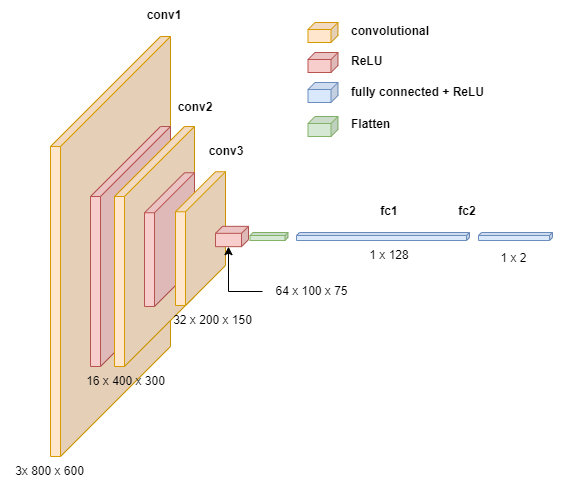
\includegraphics[width=0.8\textwidth]{assets/early-work/cnn-diagram.png}
  \caption{One of the best models for the agent reaching task}\label{fig:cnn-5050}
\end{figure}

\subsubsection{Sampling in Phases}
Another issue I ran into was the this model was performing generally well in getting very close to the target but refusing to take a very small step to collide and successfully complete the task. I realised this was because of the random sample collection being generally far away from the target, by the nature of uniform random sampling and there being vastly more space away from the target. So, to fix this, rather than changing the model architecture I changed the way expert data was sampled.

In training, I added a parameter to the training dataset, and to the creation of the training data. I made sure I could control the places data was being generated and labelling them where they were getting generated with respect to the the target. Called these phases of generation and made sure i could control the ratio of training samples and which phase they were coming from during the training. 

See Figure \ref{fig:phase-regions}, for an explanation of this idea. Giving more weighting to a closer region to the target, allowed my model to not suffer from the distribution shifts in my data, and allowed for the final push in the right direction for the agnet to complete the task successfully.

\begin{figure}[h]
  \centering
  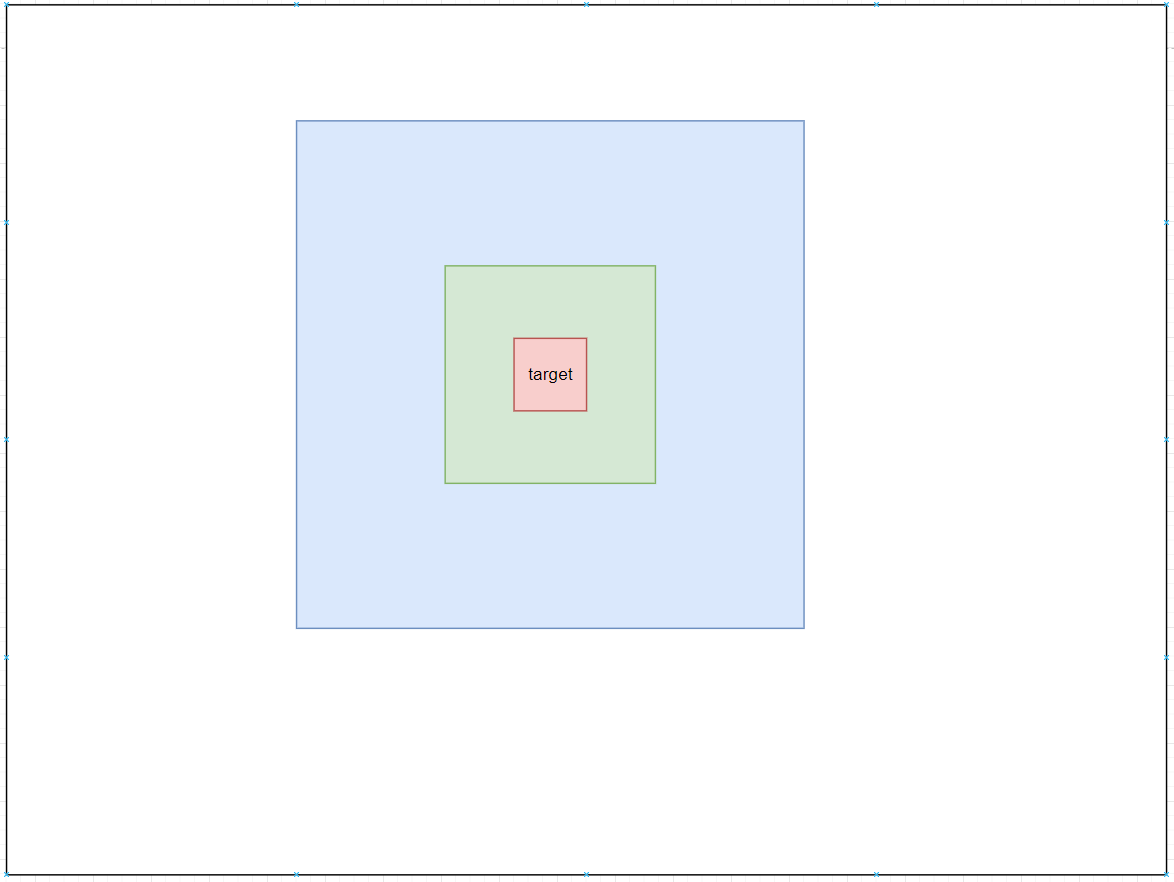
\includegraphics[width=0.8\textwidth]{assets/early-work/regions.png}
  \caption{Illustration of phases around the target, 0 would be green, 1 would be blue and 2 would be the rest of the canvas in this example. }\label{fig:phase-regions}
\end{figure}


\subsubsection{Returning to Small Blocks}
I also then got a model that was only one more convolutional layer deeper to work on the earlier smaller block size, however, the training time increase between the two were quite large for the same data sizes. Around one hour versus, four hours and change, for about 1000 episodes. Therefore, I continued this experimentation with the larger block size.


\subsection{Next Hurdle: Obstacles}
Then the next rational step was to add obstacles to simulate some ablations, which would mimic occlusions in 3D. Although, not visual barriers this was another hurdle the agent had to overcome.
Then the agent uses a path-finding algorithm, inspired by the $A^*$ algorithm \cite{cui2011based}, explores the cells around it with the heuristic of keeping the Euclidian distance of it and the target low.

\subsubsection{Obstacle Generation}
I took a simple procedural checkered approach where the canvas was divided into a grid which has cells the size of the agent. Then a cell will either be an obstacle or not with some clever mechanics around ensuring at least a single path from the agent to the target and some uncertainty. Check Figure \ref{fig:obs-gen} for some examples.

\begin{figure}[htbp]
  \centering
  \begin{subfigure}{0.45\textwidth}
      \centering
      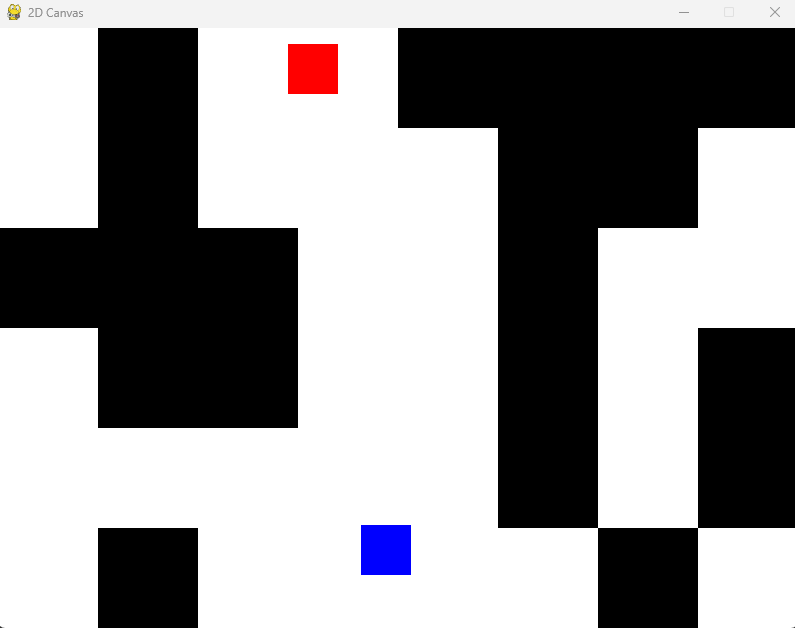
\includegraphics[width=0.8\linewidth]{assets/early-work/obs-gen1.png}
      \caption{Example 1}
  \end{subfigure}%
  \hfill
  \begin{subfigure}{0.45\textwidth}
      \centering
      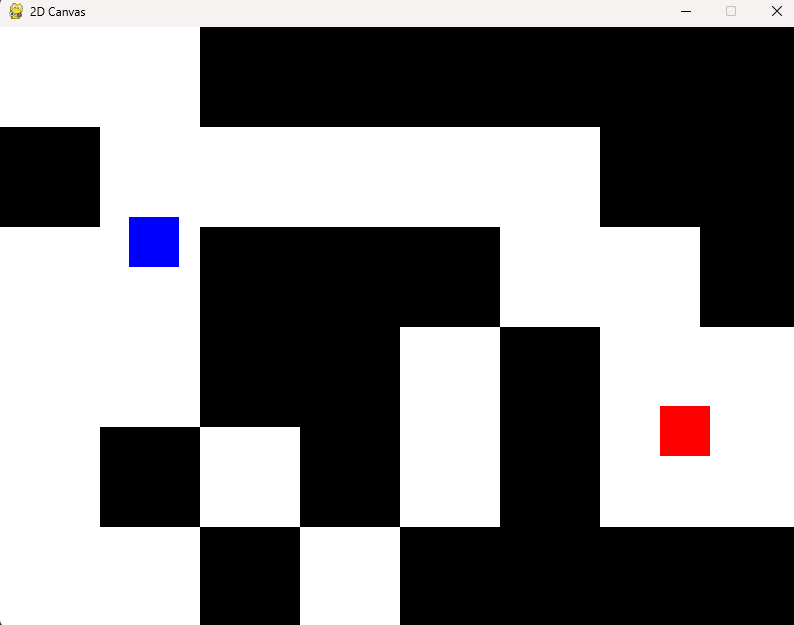
\includegraphics[width=0.8\linewidth]{assets/early-work/obs-gen2.png}
      \caption{Example 2}
  \end{subfigure}

  \vspace{0.5cm}

  \begin{subfigure}{0.45\textwidth}
      \centering
      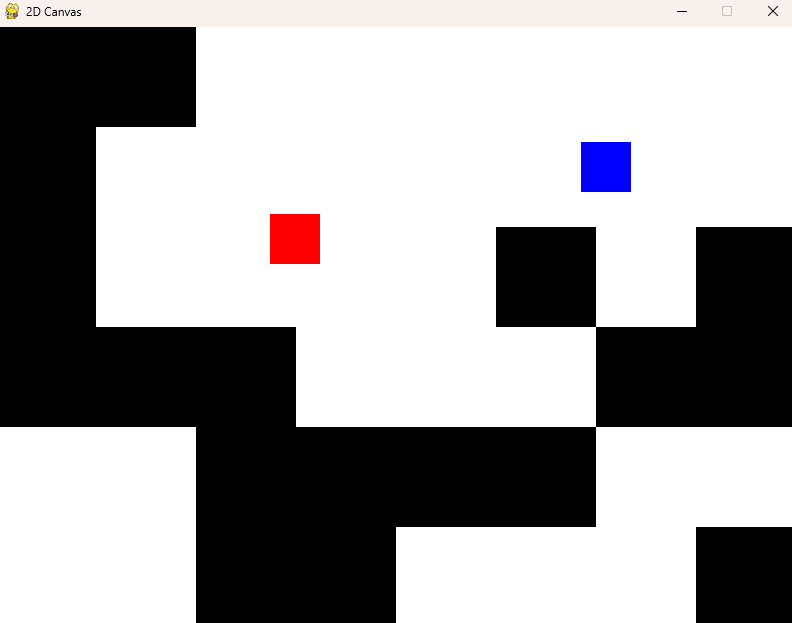
\includegraphics[width=0.8\linewidth]{assets/early-work/obs-gen3.png}
      \caption{Example 3}
  \end{subfigure}%
  \hfill
  \begin{subfigure}{0.45\textwidth}
      \centering
      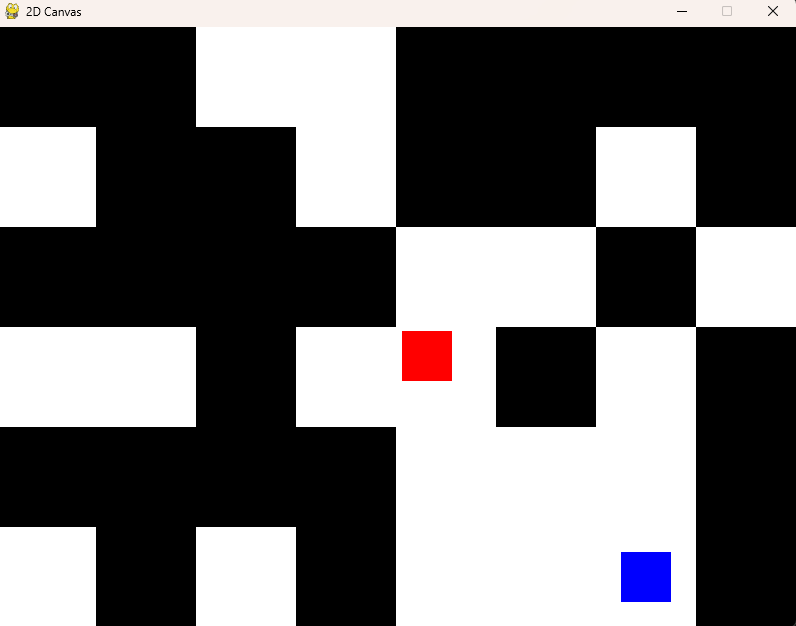
\includegraphics[width=0.8\linewidth]{assets/early-work/obs-gen4.png}
      \caption{Example 4}
  \end{subfigure}
  \caption{The 2 by 2 grid of some example obstacle generations}\label{fig:obs-gen}
\end{figure}\

\subsubsection{Getting Stuck}
I faced some issues with the model learning to avoid obstacles, the above policy for the no-obstacle case worked pretty well most of the time, however some select cases, such as there being an obstacle right between the agent and the target. 
\todo{figure for this, maybe for final report.} 

After some experimentation, I thought this might be because of the way I modelled the prediction system. Every frame expects a new movement to be generated, per the state given. This inherently has no history about where the agent was moving from. Similarly, the training data is also not ordered in any way, and it is frame corresponds to movement. Therefore, my model was essentially learning the underlying policy of the Euclidean distance heuristic used int he path finding and not extracting useful information about trajectories.

\subsubsection{Future of 2D: Sequence Models}
My next approach was to play around with a model that would take in multiple frames and output either one or multiple moves in order to have this idea of a history.

I experimented briefly with a \emph{sequence-to-model} primitively replicating a RNN, where it kept a 10 frame buffer along with the movement to predict the next movement. This idea seemed promising, however, my initial approaches were not fruitful, the models were suffering from a lot of empty episodes or repeated frames were causing erroneous learning. Therefore, I realised I had to pivot to non-concrete length sequences, such as transformer models accepting $n$ number of history frames with a max cap, rather than always needing the $x$ my fake-RNN was using (10 in my case). 

This is where I have currently left the 2D experimentation and moved onto starting some 3D approaches.

\section{3D: CoppeliaSim and RLBench}
I didn't do any meaningful work in terms of experimenting with learning or robots, but spent majority of my time setting up RLBench (quite tricky OS requirements and problems) and playing around to get myself familiar with the software.